\حصہ{فلکی سیاروں اور  مصنوعی سیاروں   کی حرکت}
اس حصہ میں ہم    قوانین نیوٹن اور قوت کشش  کی مدد سے سیاروں کی حرکت کے قوانین کپلر   اخذ کریں گے اور زمین کے گرد   مصنوعی سیاروں  کے مدار پر بحث کریں گے۔قوانین نیوٹن سے قوانین کپلر کا حصول احصاء  کی  اہم کامیابی  ہے۔اس میں وہ سب کچھ درکار ہو گا جو ہم نے اب تک پڑھا ہے جیسا فضا میں سمتیات کا الجبرا اور جیومیٹری، سمتی تفاعل  کا احصاء، تفرقی مساوات کے حل،  ابتدائی قیمت مسائل اور ترخیمی حصوں کی قطبی محددی  تشریح۔

\جزوحصہء{قطبی اور نلکی محدد میں حرکت کی سمتی مساواتیں}
ہم  یہاں  قطبی محدد  کو   \عددی{r}، \عددی{\theta} اور  نلکی محدد کو \عددی{r}، \عددی{\theta}، \عددی{z} لکھیں گے۔  ایک ذرہ قطبی محددی مستوی میں حرکت کرتا ہو، ہم اس کے مقام، سمتی رفتار اور اسراع کو متحرک اکائی سمتیات
\begin{align}\label{مساوات_سمتی_تفاعل_قطبی_روپ_الف}
\kvec{u}_r=(\cos\theta)\ai+(\sin\theta)\aj,\quad \kvec{u}_{\theta}=-(\sin\theta)\ai+(\cos\theta)\aj
\end{align}
کی روپ میں لکھتے ہیں (شکل \حوالہ{شکل_سمتی_تفاعل_قطبی_محدد_اکائی_سمتیات})۔ اکائی سمتیہ \عددی{\kvec{u}_r} کا رخ سمتیہ \عددی{\krightharpoonup{OP}} کے رخ ہے لہٰذا \عددی{\kvec{r}=r\kvec{u}_r} ہو گا۔ اکائی سمتیہ \عددی{\kvec{u}_{\theta}} بڑھتے \عددی{\theta}  کے رخ یعنی   سمتیہ \عددی{\kvec{u}_r} کو  عمودی ہے۔

\begin{figure}
\centering
\begin{minipage}{0.45\textwidth}
\centering
\begin{tikzpicture}[font=\small,declare function={f(\x)=(\x-0.5)^2-0.5;}]
\pgfmathsetmacro{\ang}{25}
\pgfmathsetmacro{\len}{2.5}
\draw[-latex](0,0)node[left]{$O$}--(3,0)node[right]{$x$};
\draw[-latex](0,0)--(0,2)node[left]{$y$};
\draw[name path=f,domain=0.6:2] plot (\x,{f(\x)});
\path[name path=r](0,0)--(\ang:\len);%coordinate(ka)node[pos=0.7,above]{$\kvec{r}$};
\draw[-latex,name intersections={of={f and r}}](0,0)--(intersection-1)node[below right]{$P(r,\theta)$}node[pos=0.5,above]{$\kvec{r}$};
\draw[-latex](intersection-1)--++(\ang:1)node[right]{$\kvec{u}_r$};
\draw[-latex](intersection-1)--++(\ang+90:1)node[left,pos=0.7]{$\kvec{u}_{\theta}$};
\draw[-stealth]([shift={(0:0.6)}]0,0) arc (0:\ang:0.6)node[pos=0.6,right]{$\theta$};
\end{tikzpicture}
\caption{نقطہ \عددی{P} کا قطبی محدد \عددی{r} سمتیہ \عددی{\kvec{r}} کی مقدار ہو گی۔یوں \عددی{\kvec{u}_r}، جو \عددی{\tfrac{\kvec{r}}{\abs{\kvec{r}}}} ہے  \عددی{\tfrac{\kvec{r}}{r}} ہو گا۔}
\label{شکل_سمتی_تفاعل_قطبی_محدد_اکائی_سمتیات}
\end{minipage}\hfill
\begin{minipage}{0.45\textwidth}
\centering
\begin{tikzpicture}[font=\small]
\pgfmathsetmacro{\ang}{25}
\pgfmathsetmacro{\len}{2.5}
\draw[-latex](0,0)node[left]{$O$}--(3,0)node[right]{$x$};
\draw[-latex](0,0)--(0,2)node[left]{$y$};
\draw[name path=f](0,-0.6) to [out=10,in=-80](2,2);
\path[name path=r](0,0)--(\ang:\len);%coordinate(ka)node[pos=0.7,above]{$\kvec{r}$};
\draw[-latex,name intersections={of={f and r}}](0,0)--(intersection-1)node[below right]{$P(r,\theta)$}node[pos=0.5,above]{$\kvec{r}$};
\draw[-latex](intersection-1)--++(\ang:1)coordinate(ka)node[below,pos=0.85]{$\dot{r}\kvec{u}_r$};
\draw[-latex](ka)--++(\ang+90:1)coordinate(kb)node[right,pos=0.7]{$r\dot{\theta}\kvec{u}_{\theta}$};
\draw[-latex](intersection-1)--(kb)node[pos=0.5,xshift=1ex]{$\kvec{v}$};
\draw[-stealth]([shift={(0:0.6)}]0,0) arc (0:\ang:0.6)node[pos=0.6,right]{$\theta$};
\end{tikzpicture}
\caption{قطبی محدد میں سمتی رفتار سمتیہ \عددی{\kvec{v}=\dot{r}\kvec{u}_r+r\dot{\theta}\kvec{u}_{\theta}} ہو گا۔}
\label{شکل_سمتی_تفاعل_سمتی_رفتار_سمتیہ}
\end{minipage}
\end{figure}

مساوات \حوالہ{مساوات_سمتی_تفاعل_قطبی_روپ_الف} سے ہمیں   درج ذیل ملتے ہیں۔
\begin{gather}
\begin{aligned}\label{مساوات_سمتی_تفاعل_قطبی_روپ_ب}
\frac{\dif\kvec{u}_r}{\dif \theta}&=-(\sin\theta)\ai+(\cos\theta)\aj=\kvec{u}_{\theta}\\
\frac{\dif\kvec{u}_{\theta}}{\dif\theta}&=-(\cos\theta)\ai-(\sin\theta)\aj=-\kvec{u}_r
\end{aligned}
\end{gather}

ہم  وقت کے لحاض سے \عددی{\kvec{u}_r} اور \عددی{\kvec{u}_{\theta}} کی تبدیلی دیکھنے کی خاطر ان  کا  تفرق \عددی{t} کے لحاض سے زنجیری قاعدہ  سے حاصل کرتے   ہیں۔
\begin{gather}
\begin{aligned}\label{مساوات_سمتی_تفاعل_قطبی_روپ_پ}
\dot{\kvec{u}}_r=\frac{\dif\kvec{u}_r}{\dif\theta}\dot{\theta}=\dot{\theta}\kvec{u}_{\theta},\quad\dot{\kvec{u}}_{\theta}=\frac{\dif\kvec{u}_{\theta}}{\dif\theta}\dot{\theta}=-\dot{\theta}\kvec{u}_r
\end{aligned}
\end{gather}
یوں سمتی رفتار (شکل \حوالہ{شکل_سمتی_تفاعل_سمتی_رفتار_سمتیہ})
\begin{align}\label{مساوات_سمتی_تفاعل_قطبی_روپ_ت}
\kvec{v}=\dot{\kvec{r}}=\frac{\dif}{\dif t}(r\kvec{u}_r)=\dot{r}\kvec{u}_r+r\dot{\kvec{u}}_r=\dot{r}\kvec{u}_r+r\dot{\theta}\kvec{u}_{\theta}
\end{align}
اور اسراع  درج  ذیل ہو گا۔
\begin{align}\label{مساوات_سمتی_تفاعل_قطبی_روپ_ٹ}
\kvec{a}=\dot{\kvec{v}}=(\ddot{r}\kvec{u}_r+\dot{r}\dot{\kvec{u}}_r)+(\dot{r}\dot{\theta}\kvec{u}_{\theta}+r\ddot{\theta}\kvec{u}_{\theta}+r\dot{\theta}\dot{\kvec{u}}_{\theta})
\end{align}

جب \عددی{\dot{\kvec{u}}_r} اور \عددی{\dot{\kvec{u}}_{\theta}} کے حصول کے لئے   مساوات \حوالہ{مساوات_سمتی_تفاعل_قطبی_روپ_پ} استعمال کیا جائے اور اجزاء کو علیحدہ کیے جائیں  تب اسراع کی مساوات   درج ذیل  صورت اختیار کرتی ہے۔
\begin{align}\label{مساوات_سمتی_تفاعل_قطبی_روپ_ث}
\kvec{a}=(\ddot{r}-r\dot{\theta}^2)\kvec{u}_r+(r\ddot{\theta}+2\dot{r}\dot{\theta})\kvec{u}_{\theta}
\end{align} 

 ہم مساوات \عددی{\kvec{r}=r\kvec{u}_r} کے دائیں ہاتھ جزو  \عددی{z\ak}  جمع کر کے ان مساواتوں کو وسعت دے کر  فضا میں حرکت کے لئے  قابل استعمال بنا سکتے ہیں۔یوں نلکی محدد میں درج ذیل ہوں گے۔
\begin{gather}
\begin{aligned}
\kvec{r}&=r\kvec{u}_r+z\ak\\
\kvec{v}&=\dot{r}\kvec{u}_r+r\dot{\theta}\kvec{u}_{\theta}+\dot{z}\ak\\
\kvec{a}&=(\ddot{r}-r\dot{\theta}^2)\kvec{u}_r+(r\ddot{\theta}+2\dot{r}\dot{\theta})\kvec{u}_{\theta}+\ddot{z}\ak
\end{aligned}
\end{gather}
دھیان رہے کہ \عددی{z\ne 0} کی صورت میں \عددی{\abs{\kvec{r}}=r} ہو گا۔

سمتیات \عددی{\kvec{u}_r}، \عددی{\kvec{u}_{\theta}} اور \عددی{\ak} دایاں ہاتھ چھوکٹ دیتے ہیں جس میں درج ذیل ہوں گے (شکل \حوالہ{شکل_سمتی_تفاعل_نلکی_تعین_گر_بنیادی_اکائی})۔
\begin{align}
\kvec{u}_r\times\kvec{u}_{\theta}=\ak,\quad \kvec{u}_{\theta}\times\ak=\kvec{u}_r,\quad \ak\times\kvec{u}_r=\kvec{u}_{\theta}
\end{align}

\جزوحصہء{سیارے مستوی میں حرکت کرتے ہیں}
نیوٹن کا قانون  تجاذب   کہتا ہے کہ  اگر سورج کی کمیت \عددی{M}، سیارہ کی کمیت \عددی{m} اور سورج  کے کمیتی    مرکز سے سیارہ کے کمیتی مرکز تک رداس سمتیہ \عددی{\kvec{r}} ہو  تب سیارہ اور سورج کے بیچ قوت کشش \عددی{\kvec{F}} درج ذیل ہو گا (شکل \حوالہ{شکل_سمتی_تفاعل_قوت_کشش_کا_رخ})  جہاں \عددی{G} (عالمگیر) \اصطلاح{تجاذبی مستقل}\فرہنگ{مستقل!تجاذبی}\حاشیہب{gravitational constant}\فرہنگ{constant!gravitational} کہلاتا ہے۔
\begin{align}\label{مساوات_سمتی_تفاعل_قوت_تجاذب_الف}
\kvec{F}=-\frac{GMm}{\abs{\kvec{r}}^2}\frac{\kvec{r}}{\abs{\kvec{r}}}
\end{align}
اگر قوت کی اکائی نیوٹن، کمیت کی اکائی کلو گرام  اور فاصلہ کی اکائی میٹر ہو تب \عددی{G=\SI{6.6720e-11}{\newton\meter\squared\per\kilo\gram\squared}} ہو گا۔
\begin{figure}
\centering
\begin{minipage}{0.45\textwidth}
\centering
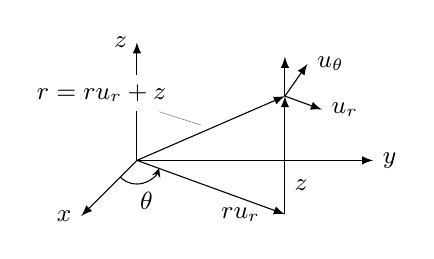
\begin{tikzpicture}[font=\small]
\pgfmathsetmacro{\len}{2}
\pgfmathsetmacro{\ang}{-20}
\draw[-latex](0,0)--++(-135:1)node[left]{$x$};
\draw[-latex](0,0)--(3,0)node[right]{$y$};
\draw[-latex](0,0)--++(0,1.5)node[left]{$z$};
\draw[-latex](0,0)--++(\ang:\len)coordinate(kB)node[pos=0.7,below]{$r\kvec{u}_r$};
\draw[-stealth]([shift={(-135:0.3)}]0,0) arc (-135:\ang:0.3)node[pos=0.6,below]{$\theta$}; 
\draw[-latex](kB)--++(0,1.5)coordinate(kT)node[pos=0.25,right]{$z\ak$};
\draw[-latex](0,0)--(kT)node[pos=0.5,pin={[fill=white,left,pin edge=-]135:{$\kvec{r}=r\kvec{u}_r+z\ak$}}]{};
\draw[-latex](kT)--++(0,0.5)node[left]{$\ak$};
\draw[-latex](kT)--++(55:0.5)node[right]{$\kvec{u}_{\theta}$};
\draw[-latex](kT)--++(\ang:0.5)node[right]{$\kvec{u}_r$};
\end{tikzpicture}
\caption{نلکی محدد میں تعین گر سمتیہ اور بنیادی  اکائی سمتیات}
\label{شکل_سمتی_تفاعل_نلکی_تعین_گر_بنیادی_اکائی}
\end{minipage}\hfill
\begin{minipage}{0.45\textwidth}
\centering
\begin{tikzpicture}
\pgfmathsetmacro{\ang}{210}
\draw[name path=oval,->-=0.8]([shift={(0:2cm and 1cm)}]0,0) arc (0:360:2cm and 1cm);
\path[name path=ray](1.25,0)--++(\ang:2.2);
\draw[-latex,name intersections={of={oval and ray}}](1.25,0)node[circ]{}node[right]{$M$}--(intersection-1)node[pos=0.25,above]{$\kvec{r}$}coordinate(kT)node[circ]{}node[above]{$m$};
\draw[opacity=0.5,very thick,-latex,gray](kT)--++(\ang:-1)node[pos=0.75,pin={[pin edge=-,fill=white,opacity=1]135:{$\kvec{F}=-\frac{GMm}{\abs{\kvec{r}}^2}\frac{\kvec{r}}{\abs{\kvec{r}}}$}}]{};
\draw[-latex](kT)--++(\ang:0.75)node[left]{$\frac{\kvec{r}}{\abs{\kvec{r}}}$};
\end{tikzpicture}
\caption{قوت کشش    دونوں کمیتوں کے بیچ سیدھے خط  پر ہو گا۔ }
\label{شکل_سمتی_تفاعل_قوت_کشش_کا_رخ}
\end{minipage}
\end{figure}
نیوٹن کے دوسرے قانون \عددی{\kvec{F}=m\ddot{\kvec{r}}}  کو مساوات \حوالہ{مساوات_سمتی_تفاعل_قوت_تجاذب_الف} کے ساتھ ملا کر
\begin{align}
m\ddot{\kvec{r}}&=-\frac{GMm}{\abs{\kvec{r}}^2}\frac{\kvec{r}}{\abs{\kvec{r}}}\nonumber\\
\ddot{\kvec{r}}&=-\frac{GM}{\abs{\kvec{r}}^2}\frac{\kvec{r}}{\abs{\kvec{r}}}\label{مساوات_سمتی_تفاعل_قوت_تجاذب_ب}
\end{align}
حاصل  ہو گا۔ سیارہ ہر لمحہ سورج کی جانب اسراع پذیر   ہے۔

مساوات \حوالہ{مساوات_سمتی_تفاعل_قوت_تجاذب_ب} کہتی ہے کہ \عددی{\kvec{r}} کا غیر سمتی مضرب \عددی{\ddot{\kvec{r}}} ہے لہٰذا 
\begin{align}\label{مساوات_سمتی_تفاعل_قوت_تجاذب_پ}
\kvec{r}\times\ddot{\kvec{r}}=\kvec{0}
\end{align}
ہو گا۔ہم دیکھتے  ہیں کہ ہ \عددی{\kvec{r}\times\ddot{\kvec{r}}}  از خود \عددی{\kvec{r}\times\dot{\kvec{r}}} کا تفرق ہے:
\begin{align}\label{مساوات_سمتی_تفاعل_قوت_تجاذب_ت}
\frac{\dif}{\dif t}(\kvec{r}\times\dot{\kvec{r}})=\underbrace{\dot{\kvec{r}}\times \dot{\kvec{r}}}_{\kvec{0}}+\kvec{r}\times\ddot{\kvec{r}}=\kvec{r}\times\ddot{\kvec{r}}
\end{align}
یوں مساوات \حوالہ{مساوات_سمتی_تفاعل_قوت_تجاذب_پ} درج ذیل کا  معادل ہے
\begin{align}\label{مساوات_سمتی_تفاعل_قوت_تجاذب_ٹ}
\frac{\dif}{\dif t}(\kvec{r}\times\dot{\kvec{r}})=\kvec{0}
\end{align}
جس کا تکمل
\begin{align}\label{مساوات_سمتی_تفاعل_قوت_تجاذب_ث}
\kvec{r}\times\dot{\kvec{r}}=\kvec{C}
\end{align}
ہے جہاں \عددی{\kvec{C}} مستقل سمتیہ ہے۔

ہمیں مساوات \حوالہ{مساوات_سمتی_تفاعل_قوت_تجاذب_ث} بتاتی ہے کہ \عددی{\kvec{r}} اور \عددی{\dot{\kvec{r}}} ہر لمحہ ایک ایسے مستوی میں ہوں گے جو \عددی{\kvec{C}} کو عمودی ہو گا۔یوں  سورج کے مرکز سے گزرتی  مستوی میں سیارے  حرکت کرتے ہیں (شکل \حوالہ{شکل_سمتی_تفاعل_سیارہ_مستوی_میں_حرکت})۔

\begin{figure}
\centering
\begin{minipage}{0.45\textwidth}
\centering
\begin{tikzpicture}
\pgfmathsetmacro{\a}{2}
\pgfmathsetmacro{\b}{1.5}
\draw(0,0)--++(\a,0)--++(45:\b)coordinate(kc)--++(-\a,0)--++(45:-\b);
\draw[-latex]($(0,0)!0.5!(kc)+(0,0.25)$)coordinate(mid)node[circ]{}node[right]{سورج}--++(0,1)node[pos=0.75,right]{$\kvec{C}=\kvec{r}\times\dot{\kvec{r}}$};
\draw([shift={(-150:1cm and 0.5cm)}]mid) arc (-150:-60:1 cm and 0.5 cm)coordinate[pos=0.25](kL);
\draw[-latex](mid)--(kL)node[pos=0.5,left]{$\kvec{r}$}node[circ]{}node[xshift=-1ex,yshift=-1ex]{سیارہ};
\draw[-latex](kL)--++(-20:0.75)node[xshift=1ex]{$\dot{\kvec{r}}$};
\end{tikzpicture}
\caption{سورج کے گرد سیارہ اس مستوی میں حرکت کرتا ہے جو \عددی{\kvec{C}=\kvec{r}\times\dot{\kvec{r}}} کو عمودی ہو اور  سورج کے کمیتی مرکز سے گزرتا ہے۔}
\label{شکل_سمتی_تفاعل_سیارہ_مستوی_میں_حرکت}
\end{minipage}\hfill
\begin{minipage}{0.45\textwidth}
\centering
\begin{tikzpicture}
\pgfmathsetmacro{\ang}{210}
\draw[name path=oval,->-=0.8]([shift={(0:2cm and 1cm)}]0,0) arc (0:360:2cm and 1cm);
\path[name path=ray](1.25,0)--++(\ang:2.2);
\draw[-latex,name intersections={of={oval and ray}}](1.25,0)node[circ]{}node[below right]{سورج}--(intersection-1)node[pos=0.5,above]{$\kvec{r}$}coordinate(kT)node[circ]{}node[below]{$P(r,\theta)$}node[above left]{سیارہ};
\draw[-latex](1.25,0)--++(1.5,0)node[below]{$\theta=0$};
\draw[-stealth]([shift={(0:0.3)}]1.25,0) arc (0:210:0.3)node[pos=0.6,shift={(135:1ex)}]{$\theta$};
\draw(2,0)node[pin=60:{\RL{حضیض شمس}}]{};
\end{tikzpicture}
\caption{حرکت سیارہ کا محددی نظام۔اوپر سے دیکھتے ہوئے حرکت، \عددی{\dot{\theta}>0} کی بنا،    گھڑی کے مخالف رخ ہے۔}
\label{شکل_سمتی_تفاعل_سیارہ_کی_حرکت}
\end{minipage}
\end{figure}
\جزوحصہء{محدد اور ابتدائی  معلومات}
ہم  نلکی محدد کے مرکز کو سورج کے  کمیتی  مرکز پر رکھتے ہیں اور سیارے کی حرکت کو  قطبی محددی سطح لیتے ہیں۔ یوں \عددی{\kvec{r}} سیارے کا تعین گر سمتیہ ہو گا  ۔یوں \عددی{\abs{\kvec{r}}=r} اور \عددی{\tfrac{\kvec{r}}{\abs{\kvec{r}}}=\kvec{u}_r} ہوں گے۔ہم  \عددی{\kvec{C}} کو محور \عددی{z} پر رکھتے ہیں لہٰذا  \عددی{\kvec{C}} کا رخ \عددی{\ak} ہو گا۔ یوں \عددی{\ak} کا \عددی{\kvec{r}\times\dot{\kvec{r}}} کے ساتھ وہی دائیں ہاتھ کا تعلق ہو گا جو اس کے ساتھ  \عددی{\kvec{C}} کا  ہے اور مثبت \عددی{z} محور سے دیکھتے ہوئے سیارہ گھڑی کے مخالف رخ گھومے   گا۔اس طرح    \عددی{t} بڑھنے سے \عددی{\theta} بڑھے گا لہٰذا تمام \عددی{t} کے لئے \عددی{ \dot{\theta}>0} ہو گا۔ہم اس لمحہ کو ابتدائی لمحہ منتخب کرتے ہیں جب سیارہ سورج کے قریب ترین ہو اور نلکی محدد کو (اگر ضرورت ہو) محور \عددی{z} کے گرد   یوں گھماتے ہیں کہ ابتدائی  لمحہ پر   \عددی{\kvec{r}}   اور  ابتدائی شعاع ہم  مکان  ہوں۔یوں ابتدائی شعاع سیارے کے  \اصطلاح{حضیض  شمس}\فرہنگ{حضیض شمس}\حاشیہب{perihelion}\فرہنگ{perihelion}  سے گزرے گا  (شکل \حوالہ{شکل_سمتی_تفاعل_سیارہ_کی_حرکت})۔

اگر ہم وقت کی پیمائش یوں کریں کہ حضیض شمسی پر \عددی{t=0} ہو تب سیارے کی حرکت کی  ابتدائی معلومات درج ذیل ہوں گی۔ 
\begin{enumerate}[a.]
\item
لمحہ \عددی{t=0} پر \عددی{r=r_0} ہو گا جو کم سے کم رداس  ہے،
\item
لمحہ \عددی{t=0} پر (\عددی{r} کی قیمت کم سے کم ہونے کی بنا)  \عددی{\dot{r}=0} ہو گا،
\item
لمحہ \عددی{t=0} پر \عددی{\theta=0} ہو گا،
\item
لمحہ \عددی{t=0} پر \عددی{\abs{\kvec{v}}=v_0} ہو گا۔\\
مزید 
\begin{align*}
v_0&=\abs{\kvec{v}}_{t=0}\\
&=\abs{\dot{r}\kvec{u}_r+r\dot{\theta}\kvec{u}_{\theta}}_{t=0}&&\text{\RL{\small{مساوات \حوالہ{مساوات_سمتی_تفاعل_قطبی_روپ_ت}}}}\\
&=\abs{r\dot{\theta}\kvec{u}_{\theta}}_{t=0}&&\text{\RL{\small{\عددی{t=0} پر \عددی{\dot{r}=0}}}}\\
&=(\abs{r\dot{\theta}}\abs{\kvec{u}_{\theta}})_{t=0}\\
&=\abs{r\dot{\theta}}_{t=0}&&\abs{\kvec{u}_{\theta}}=1\\
&=(r\dot{\theta})_{t=0}&&\text{\RL{\small{\عددی{r} اور \عددی{\dot{\theta}} دونوں مثبت ہیں}}}
\end{align*}
کی بنا ہم درج ذیل بھی جانتے ہیں۔
\item
لمحہ \عددی{t=0} پر \عددی{r\dot{\theta}=v_0} ہو گا۔
\end{enumerate}

\جزوحصہء{کپلر کا پہلا قانون  (قانون مخروط حصہ)}
کپلر کا پہلا قانون  کہتا ہے کہ  سیارے کی حرکت   مخروطی ہے جس کے ایک ماسکہ پر سورج پایا جاتا ہے۔ اس مخروط  کی سنک 
\begin{align}
e=\frac{r_0v_0^2}{GM}-1
\end{align}
اور قطبی مساوات درج ذیل ہے۔
\begin{align}
r=\frac{(1+e)r_0}{1+e\cos\theta}
\end{align}

\begin{figure}
\centering
\begin{tikzpicture}
\pgfmathsetmacro{\ang}{210}
\draw[name path=oval,->-=0.25]([shift={(0:2cm and 1cm)}]0,0) arc (0:360:2cm and 1cm)coordinate[pos=0.1](ka)coordinate[pos=0.85](kb)coordinate[pos=0.45](kc)coordinate[pos=0.51](kd);
\draw[-latex](1.25,0)node[circ]{}node[below left]{سورج}--(ka)node[circ]{}node[above]{سیارہ}node[pos=0.6,left]{$\kvec{r}$};
\draw[](1.25,0)--(kb);
\draw[](1.25,0)--(kc);
\draw[](1.25,0)--(kd);
\end{tikzpicture}
\caption{سورج اور سیارہ کے بیچ سیدھی لکیر مساوی اوقات میں مساوی  رقبوں کو واضح کرتی ہے۔}
\label{شکل_سمتی_تفاعل_مساوی_رقبہ_واضح}
\end{figure}
\جزوحصہء{کپلر کا دوسرا قانون (قانون یکساں رقبہ)}
کپلر کا دوسرا قانون کہتا ہے کہ سورج سے سیارہ تک رداسی سمتیہ ( جو ہمارے نمونہ میں   \عددی{\kvec{r}} ہو گا)مساوی اوقات میں مساوی   علاقوں کو واضح کرتا ہے (شکل \حوالہ{شکل_سمتی_تفاعل_مساوی_رقبہ_واضح})۔اس قانون کو اخذ کرنے کی خاطر  ہم مساوات \حوالہ{مساوات_سمتی_تفاعل_قطبی_روپ_ت} استعمال کرتے ہوئے  مساوات \حوالہ{مساوات_سمتی_تفاعل_قوت_تجاذب_ث} میں دی گئی حاصل صلیبی ضرب \عددی{\kvec{C}=\kvec{r}\times\dot{\kvec{r}}}   کی قیمت معلوم کرتے ہیں:
\begin{gather}
\begin{aligned}\label{مساوات_سمتی_تفاعل_کپلر_دوم_الف}
\kvec{C}&=\kvec{r}\times\dot{\kvec{r}}=\kvec{r}\times\kvec{v}\\
&=r\kvec{u}_r\times(\dot{r}\kvec{u}_r+r\dot{\theta}\kvec{u}_{\theta})&&\text{\RL{\small{مساوات \حوالہ{مساوات_سمتی_تفاعل_قطبی_روپ_ت}}}}\\
&=r \dot{r}\underbrace{(\kvec{u}_r\times\kvec{u}_r)}_{\kvec{0}}+r(r\dot{\theta})\underbrace{(\kvec{u}_r\times\kvec{u}_{\theta})}_{\ak}\\
&=r(r\dot{\theta})\ak
\end{aligned}
\end{gather}
لمحہ \عددی{t=0} پر اس سے درج ذیل حاصل ہو گا۔
\begin{align}\label{مساوات_سمتی_تفاعل_کپلر_دوم_ب}
\kvec{C}=[r(r\dot{\theta})]_{t=0}\ak=r_0v_0\ak
\end{align}
مساوات \حوالہ{مساوات_سمتی_تفاعل_کپلر_دوم_الف} میں \عددی{\kvec{C}} کی یہ   قیمت  پر کرنے سے درج ذیل حاصل ہو گا۔
\begin{align}\label{مساوات_سمتی_تفاعل_کپلر_دوم_پ}
r^2\dot{\theta}=r_0v_0\quad \text{یعنی}\quad r_0v_0\ak=r^2\dot{\theta}\ak
\end{align}
قطبی محدد میں  تفرقی رقبہ درج ذیل لکھا جاتا ہے (حصہ \حوالہ{حصہ_مخروط_قطبی_محدد_میں_تکمل})۔
\begin{align*}
\dif S=\frac{1}{2}r^2\dif \theta
\end{align*}
یوں \عددی{\tfrac{\dif S}{\dif t}} کی   قیمت ایک مستقل ہے:
\begin{align}
\frac{\dif S}{\dif t}=\frac{1}{2}r^2\dot{\theta}=\frac{1}{2}r_0v_0
\end{align} 
جو کپلر کا دوسرا قانون  ہے۔

زمین کے لئے   \عددی{r_0} تقریباً    \عددی{\SI{1.5e8}{\kilo\meter}}، \عددی{v_0} تقریباً \عددی{\SI{30}{\kilo\meter\per\second}}  ہے لہٰذا \عددی{\tfrac{\dif S}{\dif t}}تقریباً \عددی{\SI{2.25e9}{\kilo\meter\squared\per\second}} ہو گا۔یوں آپ کے دل کی ہر ایک  دھڑکن میں  زمین اپنے مدار میں  \عددی{\SI{30}{\kilo\meter}} فاصلہ طے کرتی ہے اور سورج سے زمین تک رداسی خط \عددی{\SI{2.25e9}{\kilo\meter\squared}} رقبہ واضح کرتا ہے۔ 

\جزوحصہء{کپلر کے پہلے قانون کا ثبوت}
یہ دکھانے کی خاطر کہ سورج کے گرد سیارے  کا  مدار مخروطی ہوتا ہے   جس کے ایک ماسکہ پر سورج واقع ہوتا ہے، ہمیں \عددی{r} کو متغیر \عددی{\theta} کا تفاعل لکھنا ہو گا۔ایسا کرنے کی خاطر ہمیں ایک لمبا حساب کرنا ہو گا۔ 

ہم وقتی طور پر \عددی{\dot{\theta}} سے چھٹکارا حاصل کرنے کی خاطر   مساوات \حوالہ{مساوات_سمتی_تفاعل_قطبی_روپ_ث} اور مساوات \حوالہ{مساوات_سمتی_تفاعل_قوت_تجاذب_ب} میں \عددی{\kvec{u}_r=\tfrac{\kvec{r}}{\abs{\kvec{r}}}} کے عددی سر ایک دوسرے کے برابر پر لکھ کر درج ذیل مساوات حاصل کرتے ہیں۔
\begin{align}\label{مساوات_سمتی_تفاعل_کپلر_ثبوت_پہلا_الف}
\ddot{r}-r\dot{\theta}^2=-\frac{GM}{r^2}
\end{align}
اس میں ہم  مساوات \حوالہ{مساوات_سمتی_تفاعل_کپلر_دوم_پ} سے  \عددی{\dot{\theta}} کی جگہ   \عددی{\tfrac{r_0v_0}{r^2}} پر کر کے ترتیب دیتے  ہوئے
\begin{align}\label{مساوات_سمتی_تفاعل_کپلر_ثبوت_پہلا_ب}
\ddot{r}=\frac{r_0^2v_0^2}{r^3}-\frac{GM}{r^2}
\end{align}
حاصل کرتے ہیں۔ہم متغیرات تبدیل کرتے ہوئے اس سے درجہ اول کی تفرقی مساوات حاصل کرتے ہیں۔یوں زنجیری قاعدہ  استعمال کرتے ہوئے
\begin{align*}
p=\frac{\dif r}{\dif t},\quad \frac{\dif^2r}{\dif t^2}=\frac{\dif p}{\dif t}=\frac{\dif p}{\dif r}\frac{\dif r}{\dif t}=p\frac{\dif p}{\dif r}
\end{align*}
لکھ کر مساوات  \حوالہ{مساوات_سمتی_تفاعل_کپلر_ثبوت_پہلا_ب} درج  ذیل صورت اختیار کرتی ہے۔
\begin{align}\label{مساوات_سمتی_تفاعل_کپلر_ثبوت_پہلا_پ}
p\frac{\dif p}{\dif r}=\frac{r_0^2v_0^2}{r^3}-\frac{GM}{r^2}
\end{align}
دونوں اطراف کو \عددی{2} سے ضرب کرتے ہوئے \عددی{r} کے لحاض سے تکمل لیتے ہیں۔
\begin{align}\label{مساوات_سمتی_تفاعل_کپلر_ثبوت_پہلا_ت}
p^2=(\dot{r})^2=-\frac{r_0^2v_0^2}{r^2}+\frac{2GM}{r}+C_1
\end{align}
لمحہ \عددی{t=0} پر ابتدائی معلومات \عددی{r=r_0} اور \عددی{\dot{r}=0}  سے \عددی{C_1} کی قیمت تعین ہو گی۔
\begin{align*}
C_1=v_0^2-\frac{2GM}{r_0}
\end{align*}
اس طرح مساوات \حوالہ{مساوات_سمتی_تفاعل_کپلر_ثبوت_پہلا_ت}  کو ترتیب دینے کے بعد درج ذیل لکھا جا سکتا ہے۔
\begin{align}\label{مساوات_سمتی_تفاعل_کپلر_ثبوت_پہلا_ٹ}
\dot{r}^2=v_0^2\big(1-\frac{r_0^2}{r^2}\big)+2GM\big(\frac{1}{r}-\frac{1}{r_0}\big)
\end{align}

مساوات  \حوالہ{مساوات_سمتی_تفاعل_کپلر_ثبوت_پہلا_الف} سے مساوات \حوالہ{مساوات_سمتی_تفاعل_کپلر_ثبوت_پہلا_ٹ}  حاصل کرنے میں ہم نے  \عددی{r} کی دو درجی  تفرقی مساوات سے \عددی{r}  کی ایک درجی تفرقی مساوات حاصل کی۔ ہمیں اب \عددی{\theta} کی روپ میں \عددی{r} کو  لکھنا باقی ہے   لہٰذا ہم \عددی{\theta} کو دوبارہ مساوات میں لاتے ہیں۔ایسا کرنے کی خاطر  مساوات \حوالہ{مساوات_سمتی_تفاعل_کپلر_ثبوت_پہلا_ٹ}  کے دونوں اطراف کو مساوات \عددی{r^2\dot{\theta}=r_0v_0} (مساوات \حوالہ{مساوات_سمتی_تفاعل_کپلر_دوم_پ}) کے مطابقتی اطراف سے تقسیم کر  کے حقیقت
 \عددی{\tfrac{\dot{r}}{\dot{\theta}}=\tfrac{\dif r/\dif t}{\dif\theta/\dif t}=\tfrac{\dif r}{\dif\theta}} بروئے کار لاتے ہوئے درج ذیل حاصل کرتے ہیں۔
\begin{align}\label{مساوات_سمتی_تفاعل_کپلر_ثبوت_پہلا_ث}
\frac{1}{r^4}\big(\frac{\dif r}{\dif\theta}\big)^2&=\frac{1}{r_0^2}-\frac{1}{r^2}+\frac{2GM}{r_0^2v_0^2}\big(\frac{1}{r}-\frac{1}{r_0}\big)\\
&=\frac{1}{r_0^2}-\frac{1}{r^2}+2h\big(\frac{1}{r}-\frac{1}{r_0}\big)&&h=\frac{GM}{r_0^2v_0^2}
\end{align}
اس کی مزید سادہ صورت حاصل کرنے کی خاطر  ہم درج ذیل پر کرتے ہیں۔
 \begin{align*}
u=\frac{1}{r},\quad u_0=\frac{1}{r_0},\quad \frac{\dif u}{\dif\theta}=-\frac{1}{r^2}\frac{\dif r}{\dif \theta},\quad \big(\frac{\dif u}{\dif\theta}\big)^2=\frac{1}{r^4}\big(\frac{\dif r}{\dif\theta}\big)^2
\end{align*}
یوں  درج ذیل حاصل ہو گا۔
\begin{align}
\big(\frac{\dif u}{\dif\theta}\big)^2&=u_0^2-u^2+2hu-2hu_0=(u_0-h)^2-(u-h)^2\label{مساوات_سمتی_تفاعل_کپلر_ثبوت_پہلا_ج}\\
\frac{\dif u}{\dif \theta}&=\mp\sqrt{(u_0-h)^2-(u-h)^2}\label{مساوات_سمتی_تفاعل_کپلر_ثبوت_پہلا_چ}
\end{align}

ہمیں کس علامت کا انتخاب کرنا ہو گا؟ ہم جانتے ہیں کہ \عددی{\dot{\theta}=\tfrac{r_0v_0}{r^2}} مثبت ہے۔ساتھ ہی \عددی{t=0} پر \عددی{r} کم سے کم قیمت سے شروع ہوتا ہے لہٰذا یہ یکدم گھٹ نہیں سکتا ہے، اور ابتدائی مثبت  لمحات میں \عددی{\dot{r}\ge 0}   ہو گا لہٰذا
\begin{align*}
\frac{\dif u}{\dif\theta}=-\frac{1}{r^2}\frac{\dif r}{\dif\theta}\le 0\quad\text{اور}\quad\frac{\dif r}{\dif\theta}=\frac{\dot{r}}{\dot{\theta}}\ge 0
\end{align*}
ہو گا۔مساوات \حوالہ{مساوات_سمتی_تفاعل_کپلر_ثبوت_پہلا_چ} میں منفی علامت درست ہو گی۔ یہ جاننے کے بعد ہم مساوات \حوالہ{مساوات_سمتی_تفاعل_کپلر_ثبوت_پہلا_چ} کو ترتیب دے کر  \عددی{\theta} کے لحاض سے دونوں اطراف اک تکمل لیتے ہیں۔
\begin{gather}
\begin{aligned}\label{مساوات_سمتی_تفاعل_کپلر_ثبوت_پہلا_ح}
\frac{-1}{\sqrt{(u_0-h)^2-(u-h)^2}}\frac{\dif u}{\dif\theta}&=1\\
\cos^{-1}\big(\frac{u-h}{u_0-h}\big)&=\theta+C_2
\end{aligned}
\end{gather}
چونکہ \عددی{\theta=0} پر \عددی{u=u_0}  ہو گا اور \عددی{\cos^{-1}(1)=0} ہوتا ہے لہٰذا \عددی{C_2} صفر ہو گا۔یوں
\begin{align}\label{مساوات_سمتی_تفاعل_کپلر_ثبوت_پہلا_خ}
\frac{u-h}{u_0-h}=\cos\theta
\end{align}
اور
\begin{align}\label{مساوات_سمتی_تفاعل_کپلر_ثبوت_پہلا_د}
\frac{1}{r}=u=h+(u_0-h)\cos\theta
\end{align}
ہو گا جس کو چند الجبرائی اقدام کے بعد
\begin{align}\label{مساوات_سمتی_تفاعل_کپلر_ثبوت_پہلا_ڈ}
r=\frac{(1+e)r_0}{1+e\cos\theta}
\end{align}
لکھا جا سکتا ہے جہاں 
\begin{align}\label{مساوات_سمتی_تفاعل_کپلر_ثبوت_پہلا_ذ}
e=\frac{1}{r_0h}-1=\frac{r_0v_0^2}{GM}-1
\end{align}
ہوں گے۔ مساوات \حوالہ{مساوات_سمتی_تفاعل_کپلر_ثبوت_پہلا_ڈ} اور مساوات \حوالہ{مساوات_سمتی_تفاعل_کپلر_ثبوت_پہلا_ذ} مل کر  کہتے ہیں کہ سیارے کی راہ مخروطی ہو گی جس کے ایک ماسکہ پر سورج ہو گا اور جس کی سنک \عددی{e=\tfrac{r_0v_0^2}{GM}-1} ہو گی۔ یہ قانون کپلر اول    کی جدید مساوات ہے۔


